%----------------------------------------------------------------------------------------
%	PACKAGES AND DOCUMENT CONFIGURATIONS
%----------------------------------------------------------------------------------------

\documentclass{article}


\usepackage{graphicx} % Required for the inclusion of images
\graphicspath{{figures/}}
\usepackage{subfigure} % Required for the inclusion of images
\usepackage{natbib} % Required to change bibliography style to APA
\usepackage{amsmath} % Required for some math elements 
\usepackage{listings}
\usepackage{xcolor}
\usepackage{fontspec}
\usepackage{ctex}
\usepackage{geometry}
\geometry{a4paper,scale=0.8}
\renewcommand{\contentsname}{\centerline{目录}}
\setmonofont{Consolas}
\lstset{
basicstyle=\ttfamily\footnotesize,%
escapeinside=``,%
keywordstyle=\color{black},%\bfseries, \underbar,%
identifierstyle={},%
tabsize=4,
commentstyle=\color{blue},%
stringstyle=\ttfamily,%
%labelstyle=\tiny,%
extendedchars=false,%
linewidth=\textwidth,%
numbers=left,%
numberstyle=\tiny \color{blue},%
frame=trbl%
}
%点列
%\begin{itemize}
%\item[$\bullet$]Get familiar with Y86 assembly language.
%\end{itemize}

%小标题
%\begin{center}
%{\ttfamily rsum.ys}
%\end{center}
%代码
%\begin{lstlisting}[language={[ANSI]C}]
%\end{lstlisting}
%点列和浮动体图表和ref
%\begin{itemize}
%\item[$\bullet$]{\ttfamily sum.ys} (Figure \ref{Part A: sum.ys})\\
%\end{itemize}
%\begin{figure}[htbp]%figure浮动体环境 [htbp]指定位置
%		\centering%居中排版
%		\includegraphics{A_sum}
%		\caption{Part A  {\ttfamily sum.ys}} \label{Part A: sum.ys}%标题 自动编号 label标签
%\end{figure}


%\usepackage{times} % Uncomment to use the Times New Roman font

%----------------------------------------------------------------------------------------
%	DOCUMENT INFORMATION
%----------------------------------------------------------------------------------------

\title{\textbf{操作系统课程设计Project 3\\Multithreaded Sorting Application\\ \& Fork-Join Sorting Application}} % Title

\author{姓名: 郭倩昀  
\\班级: F1903303  
\\学号: 519021910095  
\\Email: guoqianyun@sjtu.edu.cn} % Author name and email
\date{\today} % Date for the report
\begin{document}
\maketitle % Insert the title, author and date
\tableofcontents
\newpage
\section{Multithreaded Sorting Application}
\subsection{实验内容与目标}
本实验需要利用C语言设计多线程排序应用程序,主要步骤如下
\begin{itemize}
\item[$\bullet$]创建两个排序线程完成部分排序
\item[$\bullet$]创建归并排序线程完成两个排序线程结果的归并
\end{itemize}
\subsection{实验过程及步骤}
\begin{itemize}
\item[$\bullet$]设计排序线程内的排序方法\\
本人直接选用C语言<stdlib.h>带有的快速排序函数qsort(),不过重新定义了大小比较函数qsort\_compare。
\item[$\bullet$]设计归并排序线程内的归并方法\\
在函数msorting里设计归并排序。msorting根据传入的下标参数定位两段排序结果的下标,然后进行比较和归并。
\item[$\bullet$]生成待排序数组\\
main函数开始先设置随机数种子,让用户输入数组长度并选择是否随机生成数组,然后按相应方式生成待排序数组。
\item[$\bullet$]排序线程\\
根据数组大小创建相应的下标参数,创建两个排序线程sorting\_thread,用函数pthread\_create传入线程,参数和排序函数qsorting,最后用函数pthread\_join等待线程完成。
\item[$\bullet$]归并排序线程\\
同样根据数组大小创建相应归并的下标参数,创建归并排序线程merging\_thread,用函数pthread\_create传入线程,参数和排序函数msorting,最后用函数pthread\_join等待线程完成。
\item[$\bullet$]其他注意事项\\
对于每次pthread\_create,pthread\_join等关键步骤,用error变量记录完成情况,出现异常及时报错。另外,在为数组分配空间后在结束前要及时释放分配空间。
\end{itemize}
\subsection{实验代码}
\begin{center}
{\ttfamily multithreaded\_sorting.c}
\end{center}
\begin{lstlisting}[language={[ANSI]C}]
#include <stdio.h>
#include <pthread.h>
#include <stdlib.h>
#include <time.h>

int n;
int *array;
int *rst;
//quick sort for sorting_thread
int qsort_compare(const int*a, const int *b)
{
	return *a-*b;
}

void* qsorting(int *arg)
{
	if(arg[1]-arg[0]<0) return NULL;//invalid index
	qsort(array+arg[0],arg[1]-arg[0]+1, sizeof(int), qsort_compare);
	return NULL;
}
//mergesort for merging_thread
void* msorting(int *arg)
{
	int rst_dex=arg[0];
	int dex0=arg[0];
	int dex1=arg[1]+1;
	while(dex0<=arg[1]&&dex1<=arg[2])
	{
		if(array[dex0]<=array[dex1]) 
		{
			rst[rst_dex]=array[dex0];
			rst_dex++;
			dex0++;
		}
		else
		{
			rst[rst_dex]=array[dex1];
			rst_dex++;
			dex1++;
		}
	}
	while(dex0<=arg[1])
	{
		rst[rst_dex]=array[dex0];
		rst_dex++;
		dex0++;
	}
	while(dex1<=arg[2])
	{
		rst[rst_dex]=array[dex1];
		rst_dex++;
		dex1++;
	}
}

int main(void)
{
	//for random number
	srand((unsigned)time(NULL));
	int error=0;
	printf("input the array length n (0<=n<=10000): ");
	scanf("%d", &n);
	
	if(n<0||n>10000)
	{
		printf("ERROR:n is out of range\n");
		exit(1);
	}
	
	
	array=(int *)malloc(n*sizeof(int));
	rst=(int *)malloc(n*sizeof(int));
	
	char random[2];
	printf("generate the random elements?(Y/N):\n");
	scanf("%s", random);
	if(random[0]=='Y')	//generate random number
	{
		for (int i = 0; i < n; ++ i)
		{
			array[i] = rand() % 1000;
			printf("%d ",array[i]);
		}
		printf("\n");
	}
	else	//read in array
	{
		printf("input the array elements:\n");
		for(int i=0;i<n;i++)
			scanf("%d",&array[i]);
	}
	
	//Range parameter for sorting
	int parameters0[2];
	int parameters1[2];
	parameters0[0]=0;
	parameters0[1]=n/2;
	parameters1[0]=n/2+1;
	parameters1[1]=n-1;
	
	//create 2 sorting_thread
	pthread_t sorting_thread[2];
	error=pthread_create(&sorting_thread[0],NULL,qsorting,&parameters0);
	if(error)
	{
		printf("ERROR:create thread failed\n");
		exit(1);
	}
	error=pthread_create(&sorting_thread[1],NULL,qsorting,&parameters1);
	if(error)
	{
		printf("ERROR:create thread failed\n");
		exit(1);
	}
	error=pthread_join(sorting_thread[0],NULL);
	if(error)
	{
		printf("ERROR:thread join failed\n");
		exit(1);
	}
	error=pthread_join(sorting_thread[1],NULL);
	if(error)
	{
		printf("ERROR:thread join failed\n");
		exit(1);
	}
	
	
	//Range parameter for merging
	int mergeparam[3];
	mergeparam[0]=0;
	mergeparam[1]=n/2;
	mergeparam[2]=n-1;
	
	//create merging_thread
	pthread_t merging_thread;
	error=pthread_create(&merging_thread,NULL,msorting,&mergeparam);
	if(error)
	{
		printf("ERROR:create thread failed\n");
		exit(1);
	}
	error=pthread_join(merging_thread,NULL);
	if(error)
	{
		printf("ERROR:thread join failed\n");
		exit(1);
	}
	
	printf("after sorting: \n");
	for(int i=0;i<n;i++)
		printf("%d ",rst[i]);
	printf("\n");
	
	//free
	free(array);
	free(rst);
	
	return 0;
	
}
\end{lstlisting}
\subsection{实验测试}
\begin{itemize}
\item[$\bullet$]Multithreaded Sorting测试 (图 \ref{Multithreaded Sorting测试})
\begin{figure}[htbp]
		\centering
		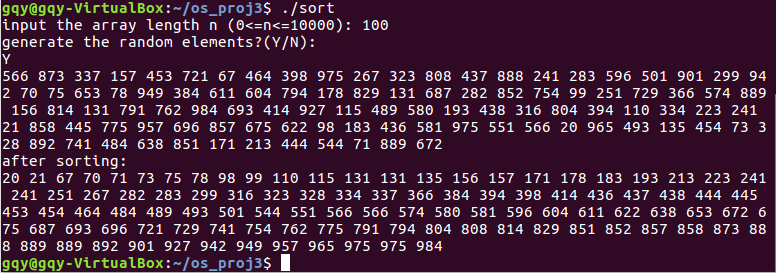
\includegraphics{mult}
		\caption{Multithreaded Sorting测试} \label{Multithreaded Sorting测试}
\end{figure}

测试指令如下
\begin{lstlisting}[language={[ANSI]C}]
gcc multithreaded_sorting.c -o ./sort -g -lpthread
./sort
100
Y
\end{lstlisting}
首先用gcc编译multithreaded\_sorting.c文件,生成sort可执行文件,加上-g -lpthread表示使用pthread API。输入./sort开始执行,输入数组长度为100,然后输入Y选择随机生成待排序数组,排序完成结果如图 \ref{Multithreaded Sorting测试}。
\end{itemize}

\section{Fork-Join Sorting Application}
\subsection{实验内容与目标}
本实验需要利用java语言设计Fork-Join排序应用程序
\begin{itemize}
\item[$\bullet$]设计归并排序版本的分治排序应用程序
\item[$\bullet$]设计快速排序版本的分治排序应用程序
\end{itemize}
\subsection{实验过程及步骤}
\noindent
归并排序
\begin{itemize}
\item[$\bullet$]创造Mergesort类\\
参考书本4.5.2中Figure4.18示例创造一个延伸RecursiveAction的Mergesort类,这里选择将THRESHOLD设置为10。
\item[$\bullet$]修改compute()函数\\
当数组大小小于THRESHOLD时候,直接采用冒泡排序完成排序工作。否则,创建新的Mergesort对象leftTask和rightTask传入相应的参数,分别调用fork(),join(),然后将leftTask和rightTask排序好的结果进行比较与归并,完成整体数组的排序。
\item[$\bullet$]生成待排序数组\\
main函数中让用户输入数组长度并选择是否随机生成数组,然后按相应方式生成待排序数组。
\item[$\bullet$]创建线程池执行任务\\
创建ForkJoinPool类型的pool,Mergesort类型的task对待排序数组创建任务,然后pool调用invoke执行任务对数组进行排序然后输出排序后数组。
\end{itemize}
快速排序(与归并排序类似)
\begin{itemize}
\item[$\bullet$]创造Quicksort类\\
参考书本4.5.2中Figure4.18示例创造一个延伸RecursiveAction的Quicksort类,这里选择将THRESHOLD设置为10。
\item[$\bullet$]修改compute()函数\\
当数组大小小于THRESHOLD时候,直接采用冒泡排序完成排序工作。否则,选中数组第一个元素作为关键值用快速排序的方式将数组分成两部分,创建新的Quicksort对象leftTask和rightTask传入相应的参数,分别调用fork(),join()。
\item[$\bullet$]生成待排序数组\\
main函数中让用户输入数组长度并选择是否随机生成数组,然后按相应方式生成待排序数组。
\item[$\bullet$]创建线程池执行任务\\
创建ForkJoinPool类型的pool,Quicksort类型的task对待排序数组创建任务,然后pool调用invoke执行任务对数组进行排序然后输出排序后数组。
\end{itemize}
\subsection{实验代码}
\begin{center}
{\ttfamily Mergesort.java}
\end{center}
\begin{lstlisting}[language=Java]
import java.util.Arrays;
import java.util.Scanner;
import java.util.concurrent.*;

public class Mergesort extends RecursiveAction {
	static final int THRESHOLD = 10;

	private int begin;
	private int end;
	private int[] array;

	public Mergesort(int begin, int end, int[] array) {
		this.begin = begin;
		this.end = end;
		this.array = array;
	}

	protected void compute() 
	{
		if (end - begin < THRESHOLD) {
			//Bubble Sort
			for (int i = end; i >= begin + 1; -- i)
			{
				for (int j = begin; j < i; ++ j)
				{
					if (array[j]>(array[j + 1])) {
						int tmp = array[j];
						array[j] = array[j + 1];
						array[j + 1] = tmp;
					}
				}
			}
		} 
		else 
		{	
			int mid = begin + (end - begin) / 2;
            //new task
			Mergesort leftTask = new Mergesort(begin, mid, array);
			Mergesort rightTask = new Mergesort(mid + 1, end, array);
			//fork and join
			leftTask.fork();
			rightTask.fork();

			leftTask.join();
			rightTask.join();

			int[] tmp = new int [end - begin + 1];
			//merge the 2 halves
			int dex1 = begin, dex2 = mid + 1, newdex = 0;
			while (dex1 <= mid && dex2 <= end) {
				if (array[dex1]<=array[dex2]) tmp[newdex++] = array[dex1++];
				else tmp[newdex++] = array[dex2++];
			}
			while (dex1 <= mid) tmp[newdex++] = array[dex1++];
			while (dex2 <= end) tmp[newdex++] = array[dex2++];

			for (int i = 0; i < newdex; ++ i)
				array[i + begin] = tmp[i];
		}
	}

	public static void main(String[] args) 
	{
		ForkJoinPool pool = new ForkJoinPool();
		Scanner sc = new Scanner(System.in);

		System.out.print("input the array length n (0<=n<=10000): ");
		int n = sc.nextInt();
		if (n < 0 || n > 10000)
		{
			System.out.println("ERROR:n is out of range");
			System.exit(1);
		}

		int[] array = new int[n];

		System.out.print("generate the random elements?(Y/N): ");
		char opt = sc.next().charAt(0);
		if (opt == 'Y') 
		{
			java.util.Random rand = new java.util.Random();
			for (int i = 0; i < n; ++ i) 
				array[i] = rand.nextInt(1000);
			System.out.print("The original array: ");
			System.out.println(Arrays.toString(array));
		} 
		else
		{
			System.out.println("input the array elements: ");
			for (int i = 0; i < n; ++ i)
				array[i] = sc.nextInt();
		}
		

		Mergesort task = new Mergesort(0, n - 1, array);
		pool.invoke(task);
		System.out.print("after sorting: ");
		System.out.println(Arrays.toString(array));
	}
}
\end{lstlisting}
\begin{center}
{\ttfamily Quicksort.java}
\end{center}
\begin{lstlisting}[language=Java]
import java.util.Arrays;
import java.util.Scanner;
import java.util.concurrent.*;

public class Quicksort extends RecursiveAction {
	static final int THRESHOLD = 10;

	private int begin;
	private int end;
	private int[] array;

	public Quicksort(int begin, int end, int[] array) {
		this.begin = begin;
		this.end = end;
		this.array = array;
	}

	protected void compute() {
		if (end - begin < THRESHOLD) {
			//Bubble Sort
			for (int i = end; i >= begin + 1; -- i)
			{
				for (int j = begin; j < i; ++ j)
				{
					if (array[j]>(array[j + 1])) {
						int tmp = array[j];
						array[j] = array[j + 1];
						array[j + 1] = tmp;
					}
				}
			}
		} 
		else 
		{
			//quick sort
			int pivot = array[begin];
			int low = begin, high = end;
			while (low < high) {
				while (low < high && array[high]>=pivot) -- high;
				if (low < high) array[low ++] = array[high];
				while (low < high && array[low]<=pivot) ++ low;
				if (low < high) array[high --] = array[low];
			}
			array[low] = pivot;
            //new task
			Quicksort leftTask = new Quicksort(begin, low - 1, array);
			Quicksort rightTask = new Quicksort(low + 1, end, array);
			//fork and join
			leftTask.fork();
			rightTask.fork();

			leftTask.join();
			rightTask.join();
		}
	}

	public static void main(String[] args) {
		ForkJoinPool pool = new ForkJoinPool();
		Scanner sc = new Scanner(System.in);

		System.out.print("input the array length n (0<=n<=10000): ");
		int n = sc.nextInt();
		if (n < 0 || n > 10000)
		{
			System.out.println("ERROR:n is out of range");
			System.exit(1);
		}

		int[] array = new int[n];

		System.out.print("generate the random elements?(Y/N): ");
		char opt = sc.next().charAt(0);
		if (opt == 'Y') 
		{
			java.util.Random rand = new java.util.Random();
			for (int i = 0; i < n; ++ i) 
				array[i] = rand.nextInt(1000);
			System.out.print("The original array: ");
			System.out.println(Arrays.toString(array));
		} 
		else
		{
			System.out.println("input the array elements: ");
			for (int i = 0; i < n; ++ i)
				array[i] = sc.nextInt();
		}
		

		Quicksort task = new Quicksort(0, n - 1, array);
		pool.invoke(task);
		System.out.print("after sorting: ");
		System.out.println(Arrays.toString(array));
	}
}
\end{lstlisting}
\subsection{实验测试}
\begin{itemize}
\item[$\bullet$]Mergesort.java测试 (图 \ref{Mergesort.java测试})
测试指令如下
\begin{lstlisting}[language={[ANSI]C}]
javac Mergesort.java
java Mergesort
100
Y
\end{lstlisting}
\begin{figure}[htbp]
		\centering
		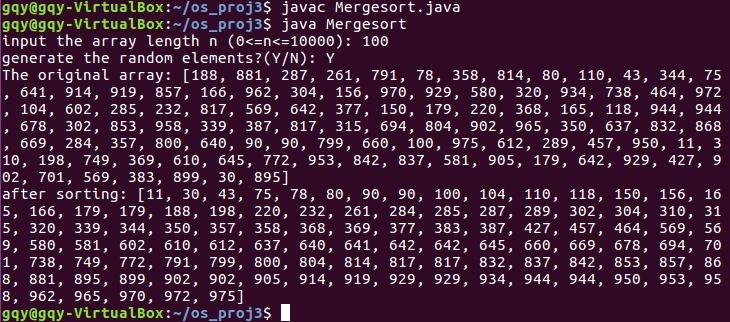
\includegraphics{ms}
		\caption{Mergesort.java测试} \label{Mergesort.java测试}
\end{figure}
首先javac Mergesort.java编译文件,输入java Mergesort执行,输入数组元素个数100,输入Y自动生成待排序数组,测试结果如图 \ref{Mergesort.java测试}。

\item[$\bullet$]Quicksort.java测试 (图 \ref{Quicksort.java测试})
\begin{figure}[htbp]
		\centering
		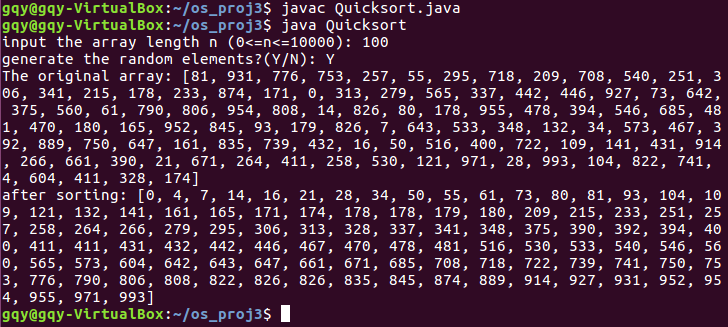
\includegraphics{qs}
		\caption{Quicksort.java测试} \label{Quicksort.java测试}
\end{figure}

测试指令如下
\begin{lstlisting}[language={[ANSI]C}]
javac Quicksort.java
java Quicksort
100
Y
\end{lstlisting}
首先javac Quicksort.java编译文件,输入java Quicksort执行,输入数组元素个数100,输入Y自动生成待排序数组,测试结果如图 \ref{Quicksort.java测试}。
\end{itemize}

\section{Conclusion}

\subsection{问题与解决方案}
本次project3的Multithreaded Sorting Application部分比较顺利,主要是掌握pthread\_create和pthread\_thread函数的使用,另外在分多线程的时候需要注意传入分任务的数组下标。

project3的另一个部分用java设计Fork-Join Sorting Application的时候,由于是新的虚拟机,首先需要配置java环境。另外由于先前对java语句没有过多的了解,在进行project的时候首先要熟悉一些必要的java语句比如输入输出生成随机数等,并且仔细参考书本的示例,进行多次尝试才最后完成了该部分的实验。

\subsection{实验心得}
本次project3让我深入体验了多线程编程,第一次使用java语言完成项目,还接触了许多新的函数工具,将多线程编程的理论知识很好地应用到实践中,在问题探索中一步步完成整个实验。总的来说本次project很好地锻炼了动手能力,并从中习得面对新事物需要勇于尝试,敢于试错,才会不断有新的收获。



%----------------------------------------------------------------------------------------


\end{document}